
%(BEGIN_QUESTION)
% Copyright 2010, Tony R. Kuphaldt, released under the Creative Commons Attribution License (v 1.0)
% This means you may do almost anything with this work of mine, so long as you give me proper credit

Compare the three force-draw curves for compound archery bows shown here:

$$\includegraphics[width=15.5cm]{i04432x01.eps}$$

Each bow exhibits the exact same peak force, holding force, and draw length.  The difference is in the shape of the cam mechanisms used to characterize each bow's draw.  Examine the three force-draw curves shown here, then answer the following questions:

\begin{itemize}
\item{} Which bow will be the more tiring (fatiguing the archer) one to shoot, all other factors being equal?
\vskip 10pt 
\item{} Which bow will accelerate the arrow most rapidly, all other factors being equal?
\vskip 10pt 
\item{} Which bow will store more energy, all other factors being equal?
\vskip 10pt 
\item{} Which bow will result in the greatest arrow velocity, all other factors being equal?
\vskip 10pt 
\item{} Which bow will be easier for a novice archer to draw, all other factors being equal?
\end{itemize}

\underbar{file i04432}
%(END_QUESTION)





%(BEGIN_ANSWER)

The answer to all questions (except the last one) is bow \#3.  Bow \#1 will be the easiest for a novice archer to draw.

%(END_ANSWER)





%(BEGIN_NOTES)


%INDEX% Mathematics, calculus: integral (work)
%INDEX% Mathematics, calculus: integration (numerical)
%INDEX% Process: archery bow force-draw curves

%(END_NOTES)


